%% Author_tex.tex
%% V1.0
%% 2012/13/12
%% developed by Techset
%%
%% This file describes the coding for rstrans.cls

\documentclass[openacc]{rstransa}%%%%where rstrans is the template name

%%%% *** Do not adjust lengths that control margins, column widths, etc. ***

%%%%%%%%%%% Defining Enunciations  %%%%%%%%%%%
\newtheorem{theorem}{\bf Theorem}[section]
\newtheorem{condition}{\bf Condition}[section]
\newtheorem{corollary}{\bf Corollary}[section]
%%%%%%%%%%%%%%%%%%%%%%%%%%%%%%%%%%%%%%%%%%%%%%%
\newcommand{\Reyn}{\mathrm{Re}}
\newcommand{\Lop}{\mathcal{L}}
\begin{document}

%%%% Article title to be placed here
\title{Generalized Quasi-linear Approximation and Non-normality in Taylor-Couette Flow}

\author{%%%% Author details
Jeffrey S. Oishi and Morgan Baxter}

%%%%%%%%% Insert author address here
\address{Department of Physics and Astronomy, Bates College, Lewiston, ME USA}

%%%% Subject entries to be placed here %%%%
\subject{xxxxx, xxxxx, xxxx}

%%%% Keyword entries to be placed here %%%%
\keywords{xxxx, xxxx, xxxx}

%%%% Insert corresponding author and its email address}
\corres{Jeffrey S. Oishi\\
\email{joishi@bates.edu}}

%%%% Abstract text to be placed here %%%%%%%%%%%%
\begin{abstract}

\end{abstract}
%%%%%%%%%%%%%%%%%%%%%%%%%%%

%%%%%%%%%% Insert the texts which can accomdate on firstpage in the tag "fmtext" %%%%%

\begin{fmtext}
\end{fmtext}
%%%%%%%%%%%%%%% End of first page %%%%%%%%%%%%%%%%%%%%%

\maketitle

\section{Introduction}
\label{sec:intro}
%Something about Taylor (1923); GQL.
Since Taylor's classic 1923 paper\cite{1923RSPTA.223..289T}, fluid between two independently rotating cylinders has become a rich laboratory for the understanding of instability, transition to turbulence, and turbulence itself. Indeed, the interplay between experiment, computation, and theoretical understanding evinced in Taylor's paper remains a model for the study of fluid dynamics.

Some of the most common forms of turbulence in nature are anisotropic, with a symmetry broken by rotation, magnetic fields, or boundary effects. In these situations, significant theoretical progress can be made by considering \emph{quasi-linear} (QL) models, in which one retains only those non-linearities that contribute to the mean flow. Recently, the generalized quasi-linear approximation (GQL) has been developed to systematically expand the QL idea to include sets of non-linear interactions between two \emph{sets} of modes, low and high, respectively, discarding those that involve only high modes (see \cite{2022arXiv220505513M} for a recent review). GQL has been shown to perform significantly better in reproducing direct numerical simulations (DNS) than QL models across a wide range of paradigm flows including forced zonal jet formation \cite{2016PhRvL.116u4501M}, rotating plane Couette flow \cite{2017JFM...810..412T}, rapidly rotating convection \cite{2018RSPSA.47480422T}, and channel flow\cite{2019Kellam}. 

Here, we consider Taylor-Couette (TC) flows at moderate inner and outer Reynolds numbers, $|\Reyn_{i,o}| < 3500$. This is an interesting testbed for GQL because it features numerous intricate patterns that are maintained by non-linear interactions beyond the typical cascade found at high $\Reyn$. 
%GQL has been show to outperform QL models in numerous highly turbulent flows, driven by $\beta$-effects on rotating spheres, rotating convection, rotating plane Couette flow (pCf, here after). 
One of the key feature of TC flow is that it has non-linear and linear instabilities in different regions of parameter space. In the linearly stable regions, transient growth has been observed in TC flow. 
As noted by \cite{2002PhFl...14.3475H}, the linear operator $\Lop$ for TC flow can be tuned to control the degree of non-normality, that is its commutator with its adjoint
\begin{equation}
    [\Lop^\dagger, \Lop] = f(\mu, \eta, \Reyn, \Gamma)
\end{equation}
can be zero or non-zero. 
This provides a very useful arena to test the validity of GQL in a system that admits both normal and non-normal operators. 

We pursue the flow into the \emph{spiral turbulence} flow regime, and consider the effectiveness of GQL in each case. The classic paper by Coles \cite{1965JFM....21..385C} was the first to note a subcritical transition to spiral turbulence when the cylinders were counter-rotating. More recent work has identified both supercritical and subcritical paths to spiral turbulence\cite{2009PhRvE..80d6315M}.
Using these prior works as a guide, we consider three cases
\begin{enumerate}
    \item Inner cylinder rotating only $\Reyn_o = 0$
    \item Counter rotating cylinders with moderate outer cylinder rotation $\Reyn_o = -1339$
    \item Counter rotating cylinders with high outer cylinder rotation $\Reyn_o = -3389$
\end{enumerate}
Case 1 has a purely normal linear operator, while the latter two feature moderate and significant non-normality respectively. 

We begin in section~\ref{sec:methods} by detailing our equations, non-dimensionalization, and numerical methods. Section~\ref{sec:linear} reviews both modal and non-modal linear analyses and contains a new analysis combining linear and non-linear aspects. In section~\ref{sec:nonlinear}, we describe the main results of the paper, the comparison of DNS, QL, and GQL in each of the three regimes. Finally, we offer discussion and concluding results in section~\ref{sec:conclusion}.
%Recently, a subcritical transition to turbulence via interpenetrating spirals has been reported \cite{2020JFM...892A..12C}. This work has a small aspect ratio $\Gamma = 5.26$, which delays the onset of linear instability to considerably higher $\Reyn_1$ for a given $\Reyn_2$. 

\section{Methods}
\label{sec:methods}
We solve the incompressible Navier-Stokes equations with unit density for $\mathbf{u}' = \mathbf{u} - \mathbf{U}$,
where $\mathbf{U} = A r + B/r \hat{\mathbf{e}}_\phi$ is circular Couette flow (CCF),
\begin{align}
\label{eqn:NS}
      \frac{\partial \mathbf{u'}}{\partial t} + \mathbf{U} \cdot \nabla \mathbf{u'} + \mathbf{u'} \cdot \nabla \mathbf{U} + \mathbf{u'} \cdot \nabla \mathbf{u'} &= -\nabla p + \nu \nabla^2\mathbf{u'}\\
      \nabla \cdot \mathbf{u'} &= 0.
\end{align}
In order to implement the GQL approximation, we introduce a projection operator to divide $\mathbf{u'}$ into two subsets,
\begin{align}
    \mathbf{u'}_l = \left< \mathbf{u'}\right>_l &= \sum_{m = -\Lambda_\theta}^{\Lambda_\theta} \sum_{k = -\Lambda_z}^{\Lambda_z} \mathbf{\hat{u}'}_{mk}(r) e^{i (m \theta + 2\pi k z/L_z)}\\
    \mathbf{u'}_h = \mathbf{u'} - \mathbf{u'}_l.
\end{align}
GQL can then be written as 
\begin{align}
\label{eqn:GQL}
      \frac{\partial \mathbf{u'}}{\partial t} + \mathbf{U} \cdot \nabla \mathbf{u'} + \mathbf{u'} \cdot \nabla \mathbf{U} +\nabla p - \nu \nabla^2\mathbf{u'} = &- \left<\mathbf{u'}_l \cdot \nabla \mathbf{u'}_l +\mathbf{u'}_h \cdot \nabla \mathbf{u'}_h\right>_l\\
      & +\left<\mathbf{u'}_l \cdot \nabla \mathbf{u'}_h + \mathbf{u'}_h \cdot \nabla \mathbf{u'}_l \right>_h\\
      \nabla \cdot \mathbf{u'} = & 0,
\end{align}
where we have written all linear terms on the left hand side. This form is equivalent to those given in prior works (for example \cite{2017JFM...810..412T}), where separate equations are written for the low and high modes, respectively.

We non-dimensionalise lengths in terms of the gap width $d = R_2 - R_1$ and velocities in terms of the inner cylinder velocity $U_i = R_i \Omega_i$. Taylor-Couette flow can be parameterised in terms of four parameters, the inner cylinder Reynolds number $\Reyn_i$, the ratio of inner to outer radii $\eta \equiv R_i/R_o$, the ratio of outer to inner rotation rates $\mu \equiv \Omega_o/\Omega_i$, and the aspect ratio of the cylinder $\Gamma \equiv L_z/d$. In our computations, the $z$ direction is periodic and thus $L_z$ is the periodicity length. We will also refer to the two Reynolds numbers $\Reyn_i$, $\Reyn_2o$, related by
\begin{equation}
    \frac{\Reyn_2}{\Reyn_1} = \frac{\mu}{\eta}.
\end{equation}
It is also quite useful to characterize times in terms of the viscous diffusion time $\tau_\nu \equiv d^2/\nu$. In our units, $\tau_\nu = \Reyn_i$.
We use the Dedalus framework (version 2) \cite{2020PhRvR...2b3068B} for all linear and non-linear calculations. Pseudospectra and critical parameters are calculated using eigentools \cite{2021JOSS....6.3079O}.
\section{Linear Stability}
\label{sec:linear}
\subsection{Non-Axisymmetric Instability with $\mu = 0$}
%HAHAH This is all laid out in Krueger, Gross, Di Prima (1966), p 523-524
%The axisymmetric test case of \cite{1984JFM...146...65M} has $\mu = 0$, $\eta = 0.875$, $\Reyn = 139.31064$, and %$k_{min} = 2\pi/L_z = 2.513$ ($L_z = 2.5$). Interestingly, table~\ref{tab:critical_m} shows that circular Couette %flow is linearly unstable to all $m \leq 4$ modes at this $\Reyn$. 
%
%A natural assumption is that one would not expect to see axisymmetric flow at these parameters. Fully non-linear %simulations initialized from very low-amplitude random, $\mathbf{\nabla \cdot u} = 0$ perturbations bear this out. %Yet, \cite{1984JFM...146...65M} makes clear reference to TVF being stable to perturbations at this flow. He also %claims that initial conditions including ``round-off noise of the computer'' lead to axisymmetric flow. This is %quite unlikely to be true. 
%
%% the two runs (axisymmetric TVF and perturbed, restarted run) are on Leavitt
%One is naturally led to the question of how axisymmetric TVF is seen in experiment if $\Reyn_{c,m=1}/\Reyn_{c, %m=0} \simeq 1.008$: $m=1$ modes are unstable at a supercriticality of less than 1\%! 
%The answer becomes obvious if one considers the usual experimental procedure: spin up a fluid from rest to a %$\Reyn < \Reyn_{c,m=0}$, allow Couette flow to be established, then spin up until the first bifurcation occurs. %Allow the TVF to settle and proceed upwards. This will indeed produce an axisymmetric TVF flow that is %\emph{itself stable against $m\ne 0$ perturbations}! At $\Reyn = 138.31$, axisymmetric TVF flow can be perturbed %with gaussian noise and will remain axisymmetric. 
%
%\begin{table}[!h]
%\caption{Critical inner $\Reyn_i$ and $k_z$ as a function of $m$ for $\eta = 0.875$, $\mu = 0$}%%%Table caption %goes here
%\label{tab:critical_m}
%\begin{tabular}{rll}%%%The number of columns has to be defined here
%\hline
%m & $\Reyn_{ic}$ & $k_z$ \\
%\hline
%0 & 118.1 & 3.12947\\
%1 & 119.0 & 3.14374\\
%2 & 121.5 & 3.18888\\
%3 & 126.17 & 3.25852\\
%4 & 133.32 & 3.35672\\
%5 & 144.20 & 3.47885\\
%\end{tabular}
%\vspace*{-4pt}
%\end{table}%%%End of the table

The axisymmetric test case of \cite{1984JFM...146...65M} has $\mu = 0$, $\eta = 0.875$, $\Reyn = 139.31064$, and $k_{min} = 2\pi/L_z = 2.513$ ($L_z = 2.5$). Interestingly, circular Couette flow is linearly unstable to all $m \leq 4$ modes at this $\Reyn$. 
In fact, linear stability analysis shows that $\Reyn_{c,m=1}/\Reyn_{c, m=0} \simeq 1.008$: $m=1$ modes are unstable at a supercriticality of less than 1\%. 
One is naturally led to the question of how axisymmetric TVF is seen in experiment!
The answer becomes clear if one considers the usual experimental procedure: spin up a fluid from rest to a $\Reyn < \Reyn_{c,m=0}$, allow Couette flow to be established, then spin up until the first bifurcation occurs. Allow the TVF to settle and proceed upwards. This will indeed produce an axisymmetric TVF flow that is \emph{itself stable against $m\ne 0$ perturbations}! At $\Reyn = 138.31$, axisymmetric TVF flow can be perturbed with gaussian noise and will remain axisymmetric. 

This is important for understanding the bifurcations from TVF to WVF: starting from $\Reyn < \Reyn_{W}$ with random initial conditions, one will find a non-axisymmetric flow.

%\subsection{$\Reyn_2 = -1000$, $\eta = 0.883$: Non-modal growth and GQL}
%Next, we look at the case of $\Reyn_2 = -1000$. Setting $\eta = 0.883$ as in Andereck et al (1986), we consider the performance of GQL in both the linearly stable and unstable regime
%\begin{itemize}
%    \item look at pseudospectra for $\Reyn_1 = 450$, $\Reyn_1 = 400$ (below and above critical)
%    \item compare pseudospectra between $\Reyn_2 = 0$ and $\Reyn_2 = -1000$
%    \item do same thing at smaller $\Reyn_2$ to compare with \cite{2002PhFl...14.3475H}
%    \item Compare GQL performance at various cutoffs
%    \item Identify non-normality parameter for TC $\Lop$ for both linearly unstable state and non-linearly modified background
%\end{itemize}
\subsection{Spiral Turbulence}
\begin{figure}
    \centering
    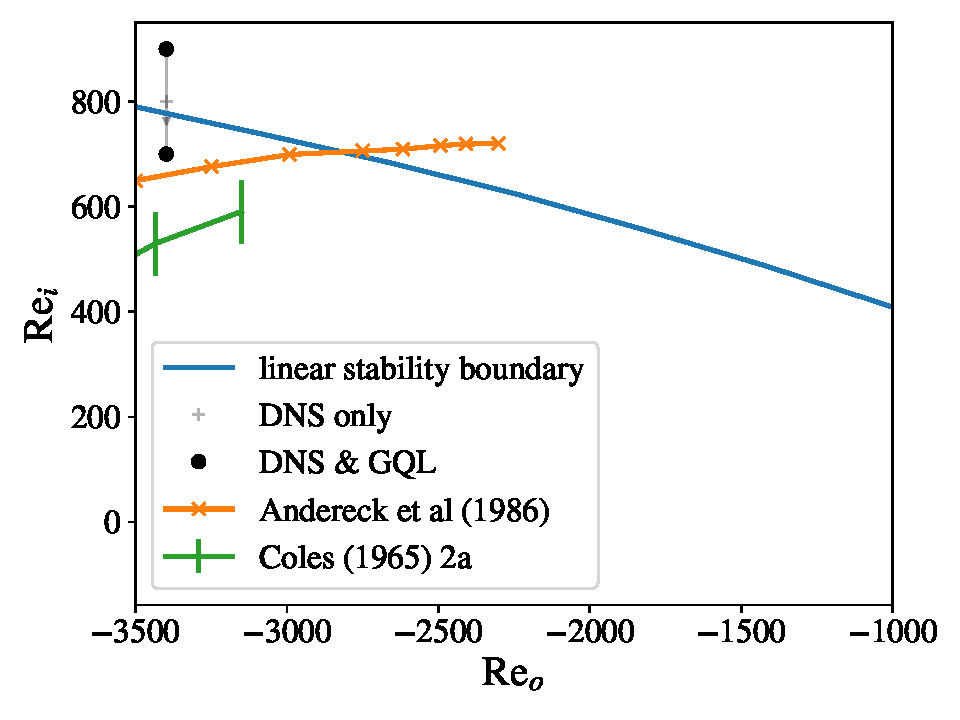
\includegraphics[width=0.8\textwidth]{../figs/reo_rei_lsb.pdf}
    \caption{A summary of spiral turbulence runs in the $\Reyn_o-\Reyn_i$ plane showing linear stability boundary. Solid circles shows points where we have conducted GQL analysis; crosses represent DNS steps along the path to subcritical behaviour. }
    \label{fig:LSB}
\end{figure}


%Meseguer et al (2009 PRE): 
%\begin{itemize}
%    \item $\Reyn_o = -1200, \Reyn_i = 600$, $\eta=0.883$, $\Gamma = 29.9$
%    \item $(N_r, N_\theta, N_z) = (20,220,220)$ HAHAHA. No way...more like $(64, 512, 512)$
%\end{itemize}

The spiral turbulence regime provides an ideal opportunity to test GQL in an environment with both spatiotemporal patterns and a tunable bifurcation: by choosing $\Reyn_i$ and $\Reyn_o$ appropriately, both subcritical and supercritical manifestations of spiral turbulence can be selected.
Following pioneering numerical work \cite{2009PhRvE..79c6309M, 2009PhRvE..80d6315M}, we set the outer cylinder rotation rate to $\Reyn_o = -3398$ for the subcritical path and $\Reyn_o = -1359$ for the supercritical path and start a series of DNS runs at a $\Reyn_i$ high enough to trigger spiral turbulence driven by linear instability from a low-amplitude, random inital condition satisfying $\nabla \cdot \mathbf{u} = 0$.
From these two seed runs, we decrease $\Reyn_i$ in steps shown in figure~\ref{fig:LSB} where each point represents a DNS or GQL simulation run for one viscous time. The solid circles in figure~\ref{fig:LSB} represent runs where we performed GQL analyses. 

\section{Results}
\label{sec:nonlinear}
%The ($\eta$, $\Gamma$) choice is motivated by \cite{1984JFM...146...45M,1984JFM...146...65M}, particularly section 4 of \cite{1984JFM...146...65M}.

First, consider a set of runs with $\mu = 0$. This is a standard, linearly unstable case. Here, we choose three $\Reyn$ values, one in the WVF flow regime $\Reyn =750$, one in the MWF $\Reyn = 1500$, and one in the TTV regime $\Reyn = 2000$. We perform two sets of runs, each varying $\Lambda = {0, 1, 2, 6, 10, 20}$ for both the $z$ and $\theta$ directions. The first set of runs is a cold start from identical initial conditions. This allows us to understand the ability of GQL to find certain flow states. The second set of runs will 

\begin{figure}
    \centering
    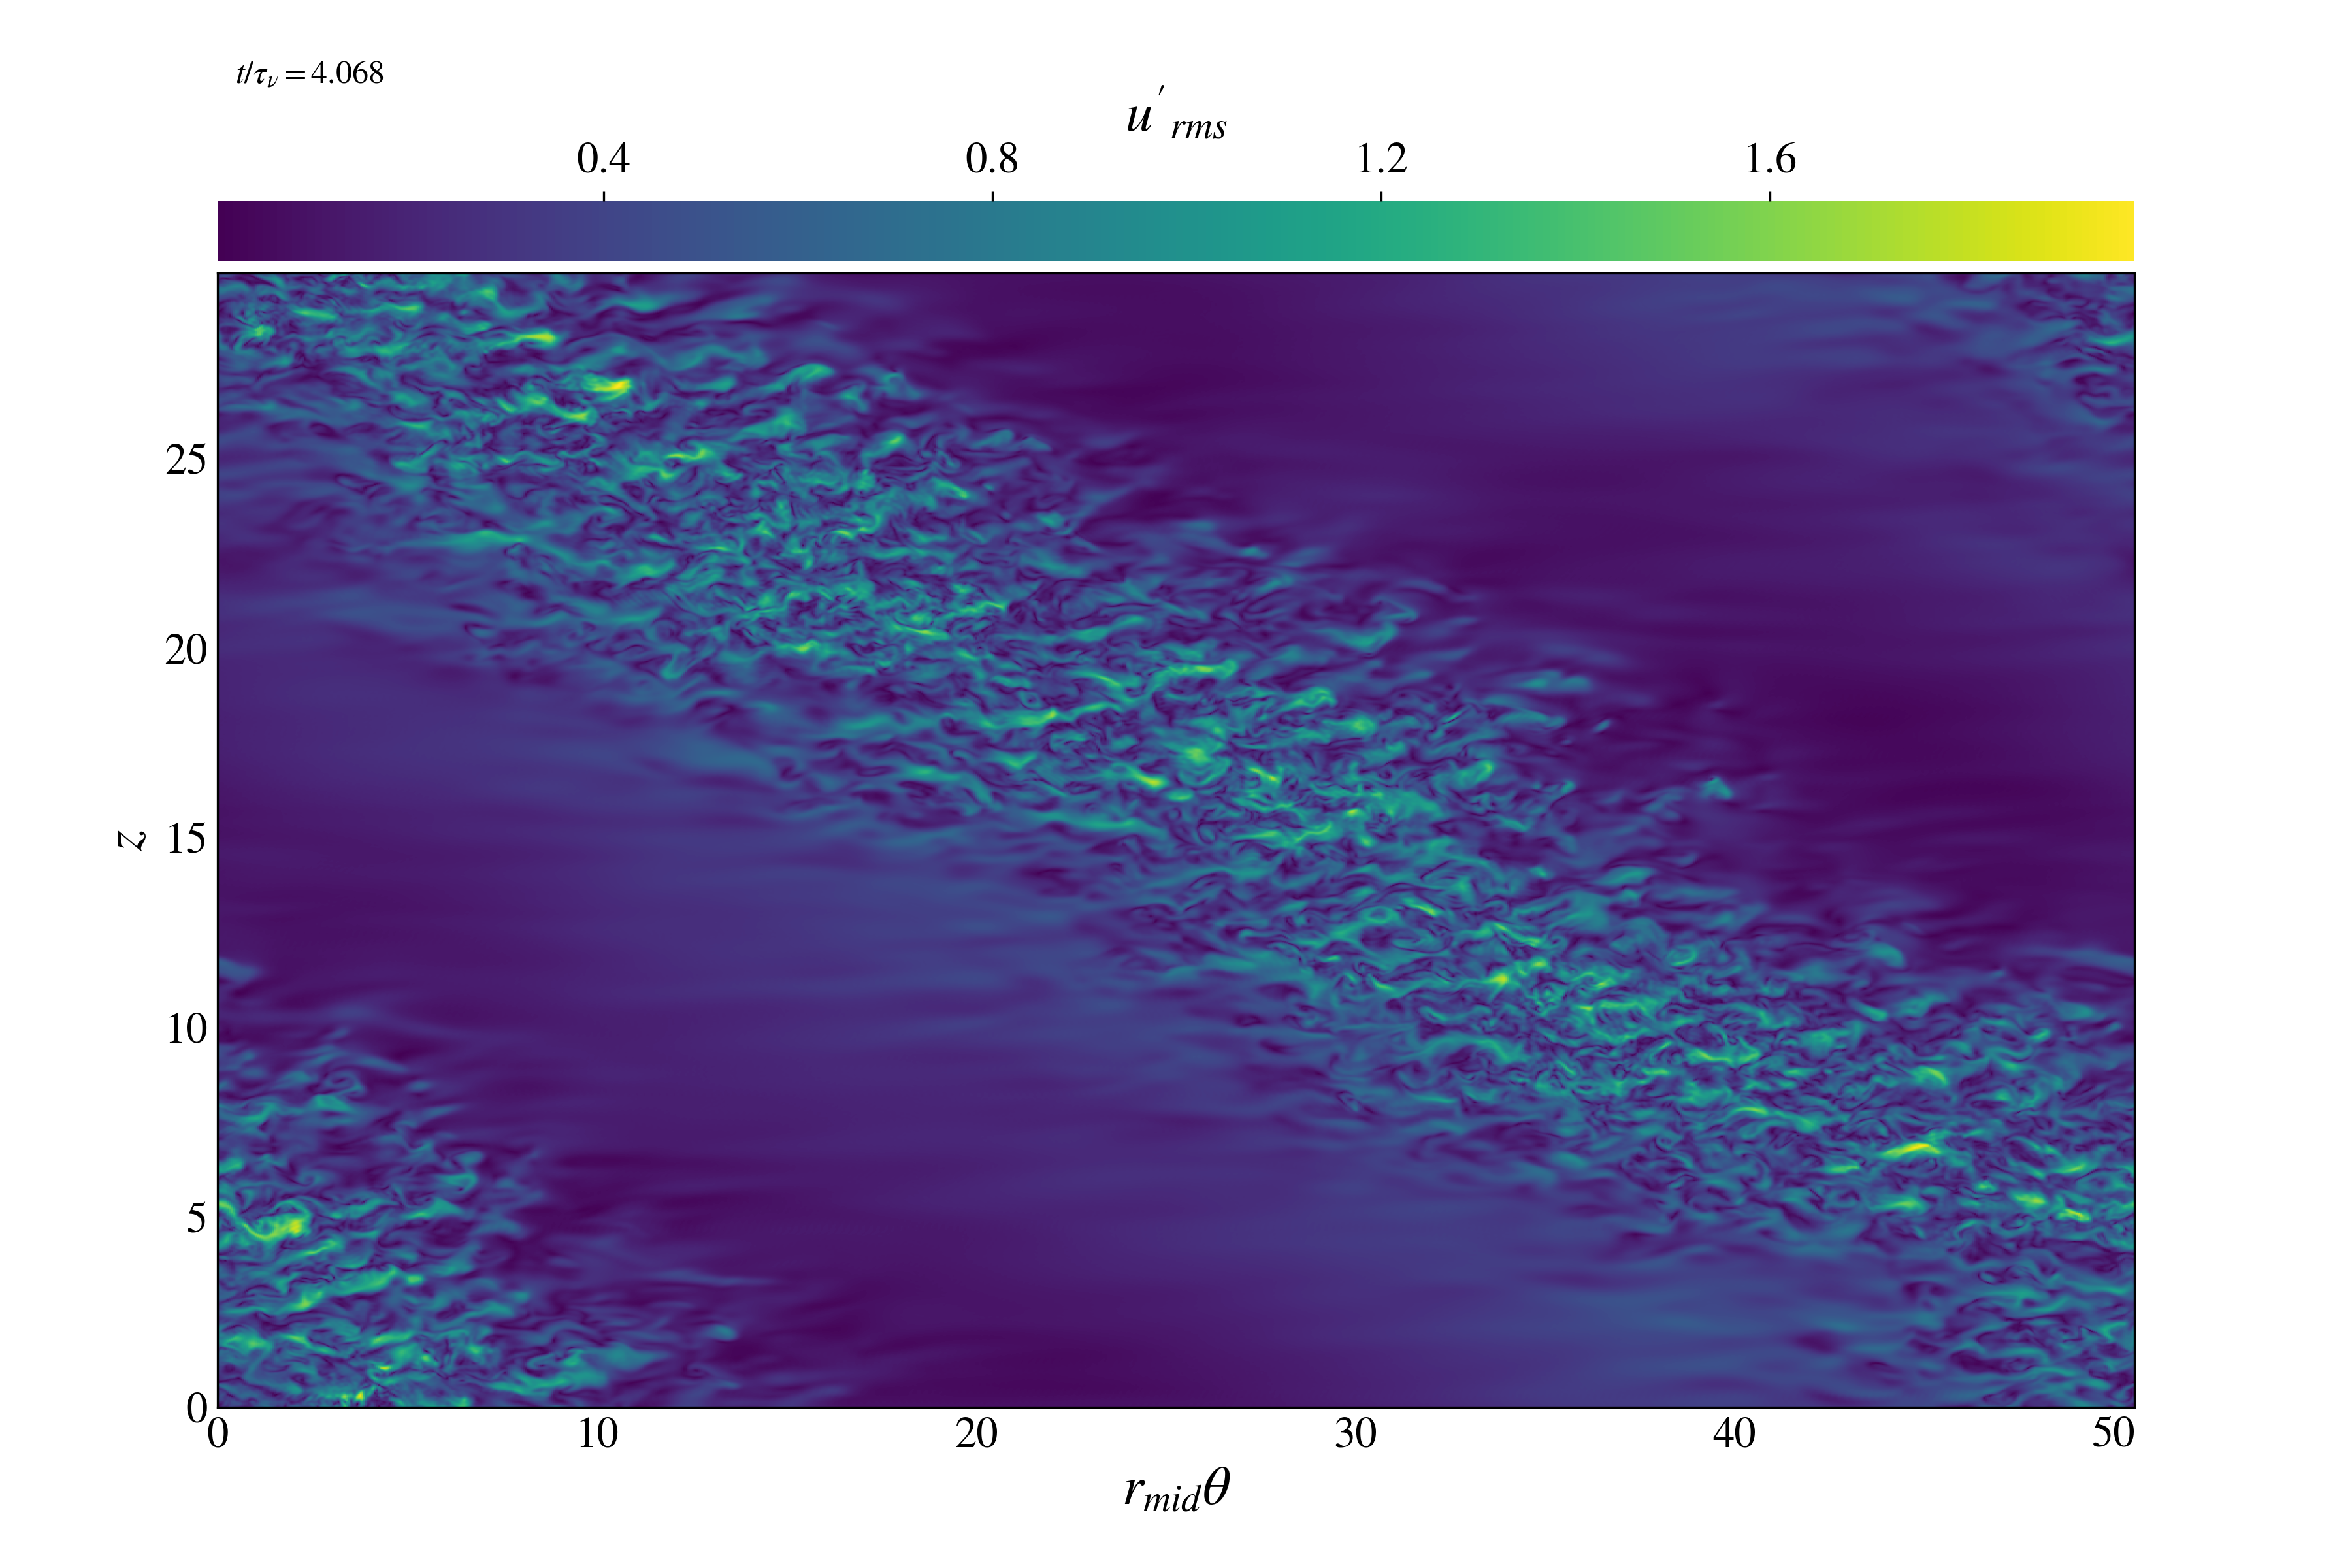
\includegraphics[width=\textwidth]{../figs/urms_tz_rei_700_reo-3398_000278.png}
    \caption{Slice of fluctuating rms velocity in the middle of the radial domain at $\Reyn_i = 700$, $\Reyn_o = -3398$. This solution is well below the linear stability threshold at }
    \label{fig:urms_tz_rei700}
\end{figure}

\begin{figure}
    \centering
    \includegraphics{}
    \caption{Caption}
    \label{fig:my_label}
\end{figure}

\begin{figure}
    \centering
    \begin{minipage}{0.45\textwidth}
        \centering
        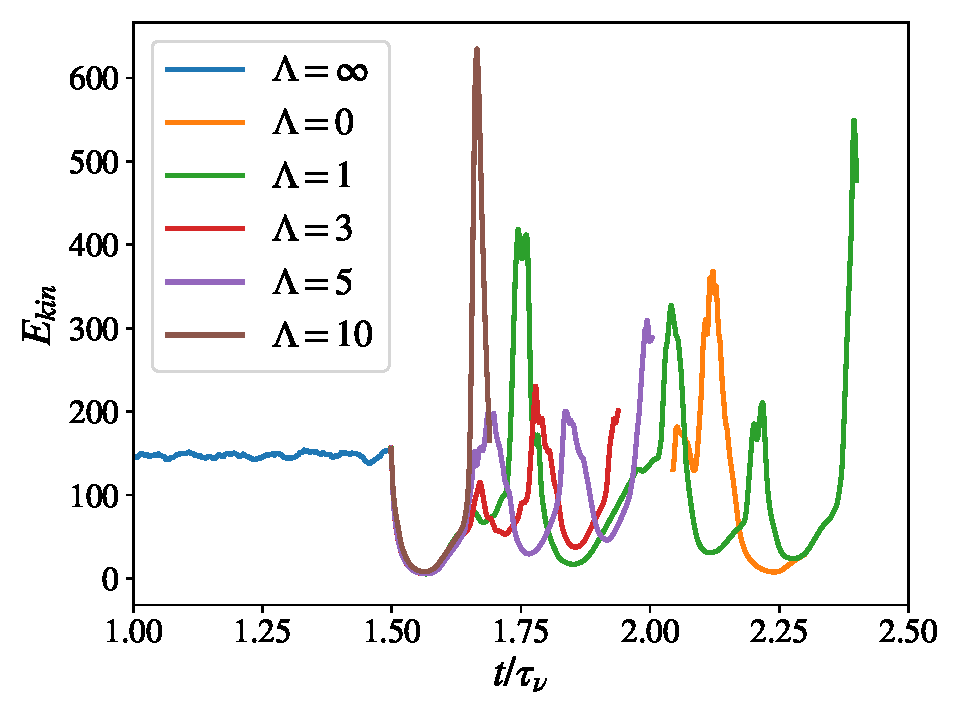
\includegraphics[width=0.9\textwidth]{figs/rei900_reo_-3398_KE_vs_t.pdf}
    \end{minipage}
    \begin{minipage}{0.45\textwidth}
        \centering
        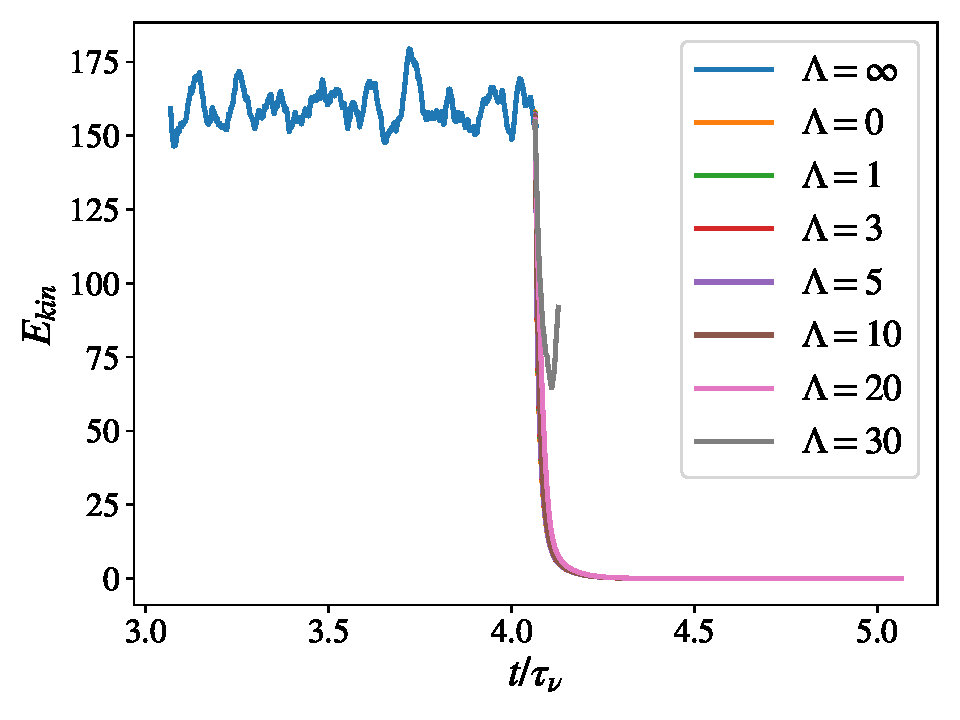
\includegraphics[width=0.9\textwidth]{figs/rei700_reo_-3398_KE_vs_t.pdf}
    \end{minipage}
    \caption{Perturbation kinetic energy as a function of time for $\Reyn_o=-3398$. On the left,  $\Reyn_i = 900$ is above the linear stability boundary, while the right shows $\Reyn_i = 700$, below the stability boundary. Starting from a saturated spiral turbulence state at $t/\tau_\nu \simeq 1.5$ (left), $t/\tau_\nu \simeq 3$ (right), we continue the solution with QL ($\Lambda = 0$) and GQL with cutoffs $\Lambda = 1,3,5,10$. For $\Reyn_i = 700$, we also use $\Lambda = 20, 30$ At higher $\Reyn_i$, all of the reduced models begin high amplitude oscillations. }
    \label{fig:ke_vs_t_rei900}
\end{figure}

\begin{figure}
    \centering
    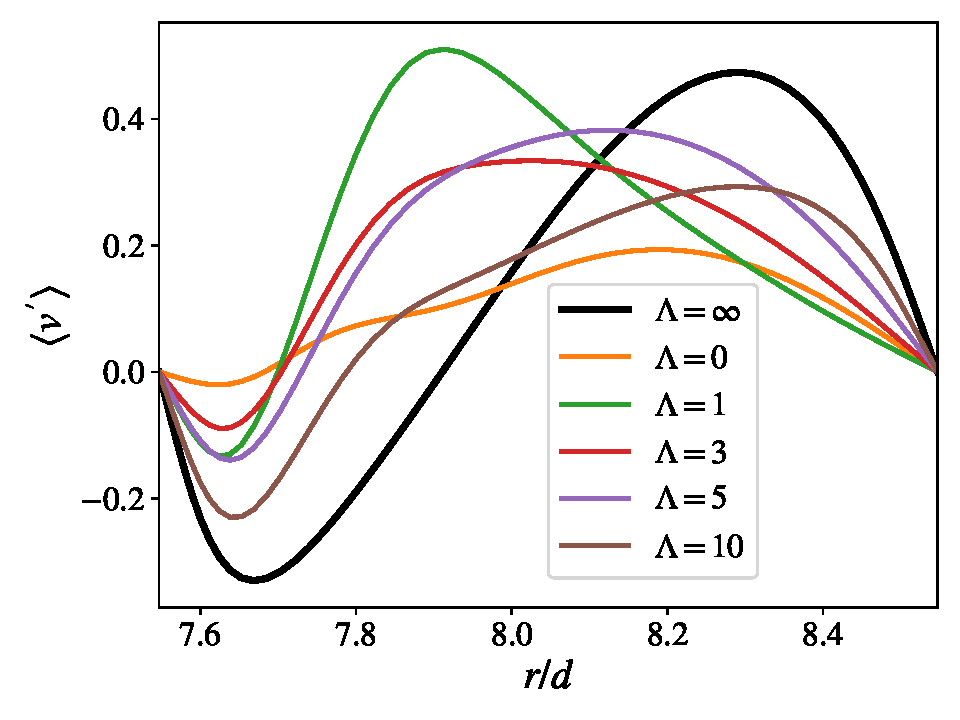
\includegraphics[width=0.9\textwidth]{figs/rei900_reo_-3398_vmean_profile.pdf}
    \caption{Mean deviation from CCF for $\Reyn_i = 900$, $\Reyn_o=-3398$. The heavy line is DNS, the orange line is QL, and all others are GQL with $\Lambda = 1,3,5,10$.}
    \label{fig:rei900_vmean}
\end{figure}

\begin{table}[!h]
\caption{Simulations}
\label{tab:simulations}
\begin{tabular}{rlllllllll}
\hline
Run & $\Reyn_i$ & $\Reyn_o$ & $\eta$ & $\Gamma$  & $N_r$ & $N_\theta$ & $N_z$& $\Lambda_\theta$, $\Lambda_z$ & Notes\\
\hline
A & 750  & 0 & 0.875  & 3 & 32 & 64 & 64 & 0, 1, 3, 5 & WVF\\
B & 1000 & 0 & 0.875 & 3 & 32 & 256 & 64 & 0, 1, 3, 5 & MWF\\
C & 2000 & 0 & 0.875 & 3 & 32 & 512 & 64 & 0, 1, 3, 5 & TTV\\
\hline
D & 900 & -3398 & 0.883 & 29.9 & 64 & 512 & 512 & 0, 1, 3, 5 & Supercritical SPT\\
E & 700 & -3398 & 0.883 & 29.9 & 64 & 512 & 512 & 0, 1, 3, 5 & Subcritical SPT\\
\hline
F & 640 & -1359 & 0.883 & 29.9 & 64 & 512 & 512 & 0, 1, 3, 5 & Supercritical SPT\\
G & 480 & -1359 & 0.883 & 29.9 & 64 & 512 & 512 & 0, 1, 5 & Supercritical IPS\\
\end{tabular}
\vspace*{-4pt}
\end{table}%%%End of the table

%\section{Resolution}
%Might compare poorly resolved DNS to low order GQL as done in\cite{2017JFM...810..412T}. Note that in poorly resolved TC DNS, one gets spurious spiral modes.

%\section{Conjugate Stable Modes}
%Conjugate stable modes? Typically, one considers the effect of the inviscid stable mode rather than the viscously damped mode. However, in the case of TC flow, the background flow profile could not be maintained by the cylinder walls in the limit $\nu \to 0$. However, because circular Couette flow is independent of $\Reyn$, probably the limit is OK? Can think about this. Obviously Rayleigh criterion applies in inviscid case, and this can be easily checked for any angular momentum profile $r^2 \Omega(r)$, so there is some merit to thinking about ideal case even in TC flow. Need to think more about this/run it by Adrian.


%The output for figure is:\vspace*{-7pt}

%\begin{figure}[!h]
%\centering\includegraphics[width=2.5in]{xxxxxx.eps}
%%% where xxxxxx name represents "figurename.eps"
%\caption{Insert figure caption here}
%\label{fig_sim}
%\end{figure}

\section{Conclusion}
\label{sec:conclusion}

%\appendix{Odds and ends}
%\begin{itemize}
%    \item On the $\Reyn_c(m=1)/\Reyn_c(m=0) %\simeq 1.008$ issue...there's a discussion in  Krueger, Gross, Di Prima (1966), p 523-524, but it references a solution in a conference proceeding that%is difficult to find. I have some memory of it being discussed in a more recent paper, but I can't find it anywhere...
%\end{itemize}
%\enlargethispage{20pt}


%\ethics{Insert ethics statement here if applicable.}

\dataccess{Insert details of how to access any supporting data here.}

\aucontribute{JSO wrote the manuscript, designed the study, wrote the GQL projection operators, and implemented the original Taylor-Couette Dedalus script. MB added the GQL terms to the TC script, developed data analysis techniques, and performed preliminary simulations. Both authors edited the manuscript.}

\competing{The authors declare that they have no competing interests.}

\funding{JSO was supported by NASA LWS grant number NNX16AC92G and NASA HTMS grant number 80NSSC20K1280. }

\ack{We thank Ben Brown for his help validating the Taylor-Couette code and John Mieszczanski for helping with resolution studies.  Computations for this paper were performed on the \emph{Leavitt} cluster at the Bates High Performance Computing Center and the NASA Pleiades system under allocation s2276.}

%%%%%%%%%% Insert bibliography here %%%%%%%%%%%%%%

\bibliographystyle{RS}
\bibliography{TC}
 
\end{document}
